%\documentclass[journal]{vgtc}                % final (journal style)
\documentclass[review,journal]{vgtc}         % review (journal style)
%\documentclass[widereview]{vgtc}             % wide-spaced review
%\documentclass[preprint,journal]{vgtc}       % preprint (journal style)
%\documentclass[electronic,journal]{vgtc}     % electronic version, journal

%% Uncomment one of the lines above depending on where your paper is
%% in the conference process. ``review'' and ``widereview'' are for review
%% submission, ``preprint'' is for pre-publication, and the final version
%% doesn't use a specific qualifier. Further, ``electronic'' includes
%% hyperreferences for more convenient online viewing.

%% Please use one of the ``review'' options in combination with the
%% assigned online id (see below) ONLY if your paper uses a double blind
%% review process. Some conferences, like IEEE Vis and InfoVis, have NOT
%% in the past.

%% Please note that the use of figures other than the optional teaser is not permitted on the first page
%% of the journal version.  Figures should begin on the second page and be
%% in CMYK or Grey scale format, otherwise, colour shifting may occur
%% during the printing process.  Papers submitted with figures other than the optional teaser on the
%% first page will be refused.

%% These three lines bring in essential packages: ``mathptmx'' for Type 1
%% typefaces, ``graphicx'' for inclusion of EPS figures. and ``times''
%% for proper handling of the times font family.

\usepackage{mathptmx}
\usepackage{graphicx}
\usepackage{times}
\usepackage{cite}
\usepackage{amsmath, amsfonts}
\usepackage{subfigure}
\usepackage{algorithm2e}
\usepackage{transparent}
\usepackage{amsthm}
\usepackage{color}
\usepackage{enumitem}
\usepackage{lipsum}
\newtheorem*{defi}{Definition}

%% We encourage the use of mathptmx for consistent usage of times font
%% throughout the proceedings. However, if you encounter conflicts
%% with other math-related packages, you may want to disable it.

%% This turns references into clickable hyperlinks.
\usepackage[bookmarks,backref=true,linkcolor=black]{hyperref} %,colorlinks
\hypersetup{
  pdfauthor = {},
  pdftitle = {},
  pdfsubject = {},
  pdfkeywords = {},
  colorlinks=true,
  linkcolor= black,
  citecolor= black,
  pageanchor=true,
  urlcolor = black,
  plainpages = false,
  linktocpage = true,
  hyperindex = true
}

%% If you are submitting a paper to a conference for review with a double
%% blind reviewing process, please replace the value ``0'' below with your
%% OnlineID. Otherwise, you may safely leave it at ``0''.
\onlineid{111}

%% declare the category of your paper, only shown in review mode
\vgtccategory{Algorithm/Technique}

%% allow for this line if you want the electronic option to work properly
\vgtcinsertpkg

%% In preprint mode you may define your own headline.
%\preprinttext{To appear in an IEEE VGTC sponsored conference.}

%% Paper title.
\title{Multiscale Symmetry Detection in Scalar Fields\\
by Clustering Contours}


%% This is how authors are specified in the journal style
\author{Dilip Mathew Thomas and Vijay Natarajan, \textit{Member, IEEE}}
\authorfooter{
% insert punctuation at end of each item
\item
 Dilip Mathew Thomas is with Department of Computer Science and Automation, Indian Institute of Science, Bangalore, India. E-mail: dilip@csa.iisc.ernet.in.
\item
 Vijay Natarajan is with Department of Computer Science and Automation, and Supercomputer Education Research Centre, Indian Institute of Science, Bangalore, India. E-mail: vijayn@csa.iisc.ernet.in.
%\item
% Martha Stewart is with Martha Stewart Enterprises at Microsoft
% Research, E-mail: martha.stewart@marthastewart.com.
}

%% indicate IEEE Member or Student Member in form indicated below
%\author{Roy G. Biv, Ed Grimley, \textit{Member, IEEE}, and Martha Stewart}
%\authorfooter{
%% insert punctuation at end of each item
%\item
% Roy G. Biv is with Starbucks Research. E-mail: roy.g.biv@aol.com.
%\item
% Ed Grimley is with Grimley Widgets, Inc.. E-mail: ed.grimley@aol.com.
%\item
% Martha Stewart is with Martha Stewart Enterprises at Microsoft
% Research. E-mail: martha.stewart@marthastewart.com.
%}

%other entries to be set up for journal
\shortauthortitle{Biv \MakeLowercase{\textit{et al.}}: }
%\shortauthortitle{Firstauthor \MakeLowercase{\textit{et al.}}: Paper Title}

%% Abstract section.
\abstract{The complexity in visualizing volumetric data often limits the scope of direct exploration
of scalar fields. Isocontour extraction is a popular method for exploring
scalar fields because of its simplicity in presenting features in the data. 
In this paper, we present a novel representation of contours with 
the aim of studying the similarity relationship between the contours. The representation 
maps contours to points in a high-dimensional transformation-invariant descriptor space. 
We leverage the power of this representation to design a clustering based algorithm for 
detecting symmetric regions in a scalar field. Symmetry detection is a challenging problem 
because it demands both segmentation of the data and identification of transformation 
invariant segments. While the former task can be addressed using topological analysis of 
scalar fields, the latter requires geometry based solutions. Our approach combines the two 
by utilizing the contour tree for segmenting the data and the descriptor space for 
determining transformation invariance. We discuss two applications, query driven exploration 
and asymmetry visualization, that demonstrate the effectiveness of the approach.
} % end of abstract

%% Keywords that describe your work. Will show as 'Index Terms' in journal
%% please capitalize first letter and insert punctuation after last keyword
\keywords{}

%% ACM Computing Classification System (CCS). 
%% See <http://www.acm.org/class/1998/> for details.
%% The ``\CCScat'' command takes four arguments.

%\CCScatlist{ % not used in journal version
%	\CCScat{Computer Graphics}{I.3.6}{Computer Graphics}{Methodology and Techniques}
%}
\teaser{
	\centering
%	\subfigure[]
%	{
		\begin{minipage}[c][1\width]{0.32\textwidth}
		{
			\centering
			\includegraphics[scale=.33]{figures/1897-full.png}
		}
		\end{minipage}
%	}
	\hspace{0.02cm}
%	\subfigure[]
%	{
		\begin{minipage}[c][1\width]{0.32\textwidth}
		{
			\centering
			\hspace{0.2cm}
			\includegraphics[scale=.31]{inkscape/descspace.pdf}
		}
		\end{minipage}
%	}	
%	\subfigure[]
%	{
		\begin{minipage}[c][1\width]{0.32\textwidth}
		{
			\centering
			\includegraphics[scale=.33]{figures/1897-sym.png}
		}
		\end{minipage}
%	}
	\caption{\label{teaser}Clustering based analysis detects symmetry at different scales 
		in a 3D cryo-electron microscopy image of AMP-activated kinase (EMDB-1897). 
		(left)~The three-fold rotational symmetry is apparent from the volume rendering. (center)~Contours 
		are represented as points in a high-dimensional shape descriptor space (illustrated in 2D). 
		Symmetric contours form a cluster in the descriptor space and can be easily identified.  
		Three such clusters are shown in gold, blue, and pink. (right)~Three symmetric regions of
		different sizes, highlighted in gold, blue, and pink, detected by the method.}
}

%% Uncomment below to include a teaser figure.
%%  \teaser{
%%  \centering
%%  \includegraphics[width=16cm]{CypressView}
%%  \caption{In the Clouds: Vancouver from Cypress Mountain.}
%%  }

%% Uncomment below to disable the manuscript note
%\renewcommand{\manuscriptnotetxt}{}

%% Copyright space is enabled by default as required by guidelines.
%% It is disabled by the 'review' option or via the following command:
% \nocopyrightspace

%%%%%%%%%%%%%%%%%%%%%%%%%%%%%%%%%%%%%%%%%%%%%%%%%%%%%%%%%%%%%%%%
%%%%%%%%%%%%%%%%%%%%%% START OF THE PAPER %%%%%%%%%%%%%%%%%%%%%%
%%%%%%%%%%%%%%%%%%%%%%%%%%%%%%%%%%%%%%%%%%%%%%%%%%%%%%%%%%%%%%%%%

\begin{document}

%% The ``\maketitle'' command must be the first command after the
%% ``\begin{document}'' command. It prepares and prints the title block.

%% the only exception to this rule is the \firstsection command
%-------------------------------------------------------------------------
\firstsection{Introduction}
\maketitle
Many scientific experiments and simulations generate scalar field data that
contain symmetric or repeating patterns. In many disciplines, 
symmetry plays an important role in studying the underlying scientific phenomena. 
For example, in crystallography, symmetry information is used to determine 
the structure of a crystal~\cite{som07}. In product design, symmetry is important 
to ensure functional efficiency and optimal manufacturing cost~\cite{booth02}. Symmetry is a 
useful cue in biology for determining growth and development of organs~\cite{stev06}. Since 
the study of symmetric features is of great interest in scientific data 
analysis, the problem of detecting symmetry in scalar fields has received 
considerable attention among researchers in the recent past~\cite{ThomN11,HongS08,kerbWKS11,ThomN13,MasoodTN13}.

Automatic detection of symmetry in scalar fields is a challenging problem and 
the quest for a widely applicable, efficient, and robust method for symmetry 
detection is ongoing. Though symmetry identification in scalar
fields is a relatively new area of research, the problem of detecting symmetry
in shapes has been well studied in the geometry processing community.
These studies have established that clustering based analyses result in superior
performance and robust identification of symmetry. Some of these methods
have been extended to scalar fields and they operate by determining symmetry
transformations through aggregation of local symmetry of sample points of the
domain. {\color{blue}Symmetry in shapes is associated with a group structure on
geometric objects that are invariant under transformations. In scalar fields, it is more
meaningful to relax this constraint and identify all repeating occurrences since this is
more useful for data exploration.} Scalar field datasets are typically represented using scalar values 
assigned to a discrete set of sample points that represent the domain under 
consideration. However, the domain and the scalar values are assumed to be continuous by
interpolating the values at the sample points. Therefore, the sample points in a scalar 
field capture the lowest level of information. In practice, scientists are more interested
in higher level features, extracted through methods like segmentation and isosurface extraction,
for studying the underlying physical phenomena. Hence, symmetry identification methods that are based on 
local information available at the sample points encounter considerable difficulty in representing 
and extracting meaningful symmetric regions. Moreover, these methods are computationally 
expensive since the number of sample points in scalar field datasets is typically orders of magnitude
higher than that in geometric shape datasets.

Though it is clear from methods proposed in the geometry processing community
that a clustering based analysis offers significant advantages in recognizing symmetry,
we believe that unlike shapes, low-level information available at the sample points of the 
domain is not suited for symmetry identification in scalar fields. In this work, we propose 
a novel symmetry detection method based on the idea of clustering contours. Isosurfaces
are extensively used in studying scalar field datasets and contours, which are 
connected components of isosurfaces, capture information 
about a scalar field at a macroscale.
Therefore, contours are more suitable for a clustering based analysis as opposed to sample 
points of the domain. It is easy to see that contours
belonging to regions with symmetric scalar field distribution are also symmetric. Using an 
appropriate shape descriptor, our method maps contours to points in a descriptor space 
such that the distance between points in the descriptor space is a measure of similarity 
between the contours. As a result, points in the descriptor space 
representing symmetric contours lie in close 
proximity to each other and form clusters in the descriptor space. The region of the domain
corresponding to each such contour can be extracted and these regions
are reported as symmetric. Note that the choice
of the shape descriptor is not fixed and depending on the noise characteristics and the definition
of similarity relevant to the application of interest, an appropriate descriptor may be used.
Figure~\ref{teaser} illustrates our approach on a 3D cryo-EM image of AMP-activated kinase (EMDB-1897) 
with three-fold rotational symmetry. {\color{blue}Our method identifies symmetric regions of different
scales. The large-scale features shown in gold and the small-scale features shown in blue and pink
highlight the multiscale aspect of our approach.}

The main contributions of this paper are the following:
\begin{itemize}[itemsep=0mm]
%\vspace{-0.25cm}
\item A formulation of the problem of symmetry detection in scalar fields
as a clustering problem in a shape descriptor space. This model
provides a lot of flexibility in analysing similarity of scalar fields
as well as handling noise since it allows the shape representation and the 
descriptor space to be varied.
%\vspace{-0.25cm}
\item A novel representation of contours as points in a contour descriptor space.
Similarity between contours is naturally defined as the distance between points 
in this space. This is a generic representation of independent interest 
and we show its benefit in similarity analysis of scalar fields.
%\vspace{-0.25cm}
\item A robust algorithm to detect symmetric regions at multiple scales. Though geometry based 
symmetry detection methods are typically computationally costly, we design an efficient algorithm 
that employs elegant optimisations by incorporating topological information 
about the contours using the contour tree.
%\vspace{-0.25cm}
\item Applications to query driven exploration and asymmetry visualization.
\end{itemize}
Symmetry information in scalar fields
has been used for transfer function design, exploration of isosurfaces, selection of cross-section
planes and view directions, linked selection and editing, query driven exploration,
and visualization of features through dual rendering~\cite{ThomN11,HongS08,ThomN13,MasoodTN13}.
We believe that as better techniques for symmetry detection are developed,
many more applications will emerge.
\section{Related Work}
Existing symmetry identification methods in scalar fields can be broadly classified into two
categories, namely, geometry based methods and topology based methods. We briefly review
these methods in this section.
\subsection{Geometry based approaches}
Several methods have been proposed in the literature for detecting
symmetry in shapes as described in the survey paper by
Mitra~et~al.~\cite{MitPWC2012}. Some of these methods~\cite{Mitra06,KazhdanCDFR03,BokBWSS09} have 
been applied to scalar fields~\cite{MasoodTN13,HongS08,kerbWKS11}. However, they struggle to address 
the challenges in extending geometric methods to scalar fields.
Scalar field datasets are significantly larger in size and hence symmetry detection is computationally costly.
Geometric methods typically consider geometric information derived from a small region around each sample
point of the domain for symmetry recognition. A direct extension of this approach to scalar fields
suffers from the difficulty of capturing important features and leads to poor performance 
in extracting higher level features and handling of noise in the data.
Moreover, the scalar field is considered to be continuous over the domain by interpolating the values at 
the discrete set of sample points. Inspecting only the sample points
introduces additional challenges due to discretization errors since the symmetric counterpart for a 
given point may be an interpolated point.

Hong and Shen~\cite{HongS08} propose a method to detect global reflective symmetry by identifying planes
of reflection that minimize the difference between the scalar value at a point and its
reflection. This method is computationally inefficient and cannot be easily extended to identify 
other types of symmetry. Kerber~et~al.~\cite{kerbWKS11} build a graph network of crease line features 
and detect symmetry by computing transformations that match subgraphs within the crease line network.
Since only a small subset of features in scalar fields contain crease lines, 
this method is not very useful in practice. Masood~et~al.~\cite{MasoodTN13} detect
symmetry by identifying symmetry transformations as clusters in the space of all transformations.
The clusters are generated by aggregating local symmetry transformations of pairs of points in the 
domain. This method relies on local signatures of sample points for determining 
transformations and as a result several parameters need to be tweaked at various stages of 
the symmetry detection pipeline to limit the adverse effects of variations in the local signatures 
and discretization errors.  Moreover, the transformation space often contains additional transformations
that introduces artifacts. The above methods compute transformations between 
candidate pairs for identifying symmetry and are computationally costly. Moreover, they 
are driven by purely local geometric measures and do not incorporate any criterion 
to either recognize important features or discard pairs corresponding to noise. 
Our method, on the other hand, uses topological information derived from the contour tree to infer 
importance of a feature and this allows the design of a feature-aware algorithm for symmetry identification. 

Bruckner~et~al. propose an information theoretic approach for isosurface similarity 
detection~\cite{BrucknerM10,haidacher11}. This method uses mutual information between distance 
transforms to quantify the information common to two isosurfaces and builds a similarity map 
between all pairs of isosurfaces. Clusters with high mutual information correspond to
similar isosurfaces both within and across datasets. {\color{blue}While this method is related since
it is also based on isosurface similarity, their goal is to select a subset of isovalues
which are important. They use distance transforms to identify redundant isovalues by
computing similar family of isosurfaces that form an onion-peel like layered arrangement. 
The goal of our method, on the other hand, is to locate regions which are similar and hence
we compute similarity between contours and not isosurfaces.} While the isosurface similarity map based
method is limited to analysing similarity between pairs of datasets, the descriptor space can 
be used to analyse multiple datasets simultaneously. Similarity between different scalar 
fields has also been studied by measuring the extent of overlap
between contours~\cite{SchneiderWCHS08,schn13}. The distance transform
descriptor and the overlap measure are affected by changes in orientation.
Our method is not restricted to a particular choice of descriptor. Based on the requirements of 
the application under consideration, our method  can be adapted to be sensitive or 
insensitive to orientation. 
\subsection{Topology based methods}
Thomas and Natarajan propose topology based methods for symmetry identification and these methods 
are computationally efficient because they operate on graph representations of the scalar field
like the contour tree~\cite{ThomN11} and the extremum graph~\cite{ThomN13}. The contour tree based method 
assumes that the subtrees of the contour tree corresponding to symmetric regions are structurally
similar. They detect symmetry by evaluating structural similarity between the subtrees using a 
similarity score that measures the overlap between the branches of the trees. 
This method can find symmetry at multiple scales but cannot handle
noise that destroy the repeating structure of the subtrees. The extremum 
graph based method selects a set of extrema called seed set and 
estimates distances robustly through a graph traversal procedure. A carefully chosen distance 
threshold is used to disconnect the graph and classify the seeds into different groups called 
super-seeds. A region growing procedure is then used to identify the symmetric region 
corresponding to each super-seed. This procedure makes a strong assumption that the symmetric regions
can be identified purely from the proximity relationship between the seeds. Hence,
it relies heavily on a meaningful selection of seed set which involves significant effort 
and understanding about the symmetry of the domain. In addition, this method requires several thresholds
to be set.

The above methods being topological in nature do not ensure that the regions reported by
them are indeed geometrically symmetric while our method being geometric in nature, 
ensures that the regions extracted are symmetric. Moreover, current methods compare candidate regions 
pairwise and rely on a similarity threshold to classify them into symmetric groups. Determining
the similarity threshold is a challenge when using datasets with varying characteristics.
Clustering based analysis avoids the need for pairwise comparisons. Instead, the symmetric regions
are directly obtained as clusters in the descriptor space. 
Similarity between scalar fields have been
studied in the context of shape matching applications by using graph matching methods on 
discrete approximations of the contour tree~\cite{ZhangBKDNB06,HilagaSKK01}.
The contour tree provides metadata information about the contours
and allows integration of topological information in geometric processing. Thus, by utilizing 
the descriptor space to capture geometric information about contours together with the power of 
the contour tree as a topological abstraction of contours, our method offers significant advantages over 
existing symmetry identification methods. 
\begin{figure}[b]
	\centering
	{
		\centering
		\begin{minipage}[c][2.4cm][b]{0.4\linewidth}
			{
				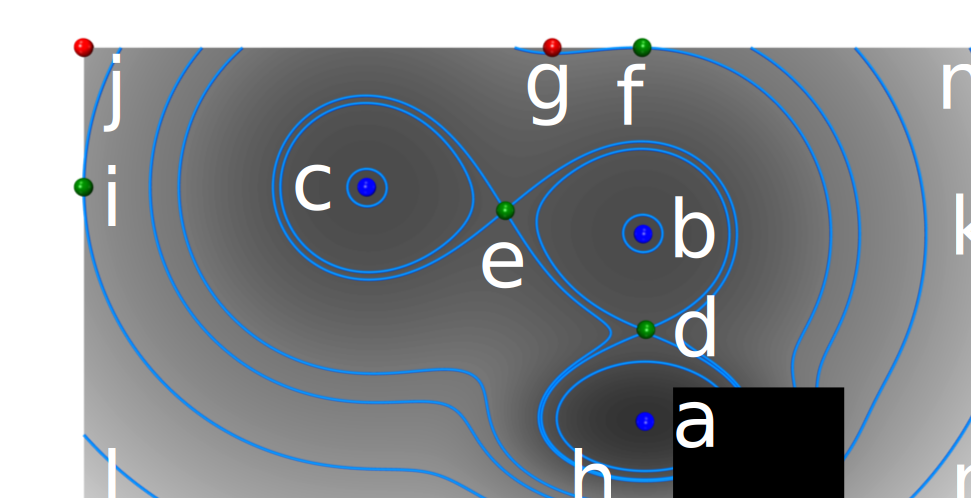
\includegraphics[scale=0.15]{inkscape/ctfield.pdf}
			}
		\end{minipage}
	}
	{
		\centering
		\hspace{1cm}
		\begin{minipage}[c][2.45cm][b]{0.3\linewidth}
			{
				
\includegraphics[scale=0.15]{inkscape/ct.pdf}
			}	
		\end{minipage}
	}
	\caption{\label{ct}The contour tree captures changes in the topology of the level sets of a scalar field. 
	(left)~A scalar field and its level sets. (right)~The corresponding contour tree. The red nodes are
	local maxima, the blue nodes are local minima, and the green nodes are saddles.}
\end{figure}
\section{Definitions}
Consider a \emph{scalar field}, $f : \mathbb{M}  \rightarrow \mathbb{R}$, defined on a 
simply connected domain $\mathbb{M}$. The preimage of $f$ for a given value $u \in \mathbb{R}$, 
$f^{-1}(u)$, is called a \emph{level set} of $f$. A level set may have multiple components
and each component is called a \emph{contour}. Consider a sweep of the domain using level sets in the order
of increasing function values. A contour is created at a \emph{minimum}, may merge
with another contour at a \emph{join saddle} or split into different contours at a \emph{split saddle}, 
and is destroyed at a \emph{maximum}. The \emph{contour tree} is a topological 
data structure that captures these changes in the connectivity of the level sets, see Figure~\ref{ct}.
Let $R$ be an equivalence relation defined on points in $\mathbb{M}$: $xRy$ for $x,y 
\in \mathbb{M}$  if $x,y$ belong to the same contour. The contour tree is the quotient space 
induced by this relation. 

Subdomains $\mathbb{M}_1, \mathbb{M}_2 \subseteq \mathbb{M}$ are said to be \emph{symmetric} 
if there is a transformation $T$ such that ${\mathbb{M}_2=T(\mathbb{M}_1)}$ and 
${f(x)=f(T(x))}$ for all $x \in \mathbb{M}_1$. If $c_1$ and $c_2$ are contours of the same level
set that belong to $\mathbb{M}_1$ and $\mathbb{M}_2$ respectively, it is easy to see that if 
$\mathbb{M}_1$ and $\mathbb{M}_2$ are symmetric then $c_1$ and $c_2$ are also symmetric. 
We make use of this property and detect symmetric subdomains by identifying symmetry of the 
contours belonging to the subdomains. The above definition of symmetry requires computation of the symmetry 
transformation $T$, which is a costly operation. Therefore, we use an alternate definition of symmetry.
Let $\mathbb{C}$ be the set of all contours. 
Consider a function $g : \mathbb{C} \rightarrow \mathbb{R}^n$ such that $g(c) = g(T(c))$
where $T$ is a transformation. In other words, $g$ is a function that maps each
contour to a point in a high-dimensional space such that a contour and its 
copies are mapped to the same point. {\color{blue}The contours which are mapped to the same
point need not form a symmetry group. Instead, all repeating instances of a contour
are mapped to the same point.} The point to which a contour is mapped is called a 
\emph{descriptor} and the high-dimensional space is called the \emph{descriptor space}, see Figure~\ref{ctmap}. 
For illustration, the descriptor space is shown in 2D but the actual dimension of the space
depends on the choice of the descriptor. The distance between contours in the descriptor space is a
measure of their similarity. In practice, scalar fields do not exhibit perfect symmetry and therefore
it is important to detect symmetry in an approximate sense. Ideally, deviation
from perfect symmetry should be measured in the space of shapes but 
it is more convenient to measure deviations in the descriptor space. If contours $c_1$ and 
$c_2$ are not perfectly symmetric, then $c_1$ and $c_2$ will not be mapped
to the same point in the descriptor space. The distance between
the contours in the descriptor space, $\lVert g(c_1)-g(c_2) \rVert$, will be indicative
of the deviation from perfect symmetry. 
\begin{defi}[Symmetric Contours]
Contours $c_1$ and $c_2$ are perfectly symmetric if $\lVert g(c_1)-g(c_2) \rVert = 0$,
where $\lVert \cdot \rVert$ is a norm in the descriptor space. They are 
{$\epsilon$-symmetric} if $\lVert g(c_1)-g(c_2) \rVert \leq \epsilon,$ for $\epsilon > 0$.
\end{defi}
Shape descriptors have been extensively used in the
geometry processing community for shape matching and there is a
vast collection of research papers in this 
area~\cite{lian2013,van2011,tangelder2008survey,qin2008content}. 
It is possible that a shape descriptor may incorrectly map contours $c_1$ and 
$c_2$ to the same point even when they have totally different shapes. A good shape descriptor should 
discriminate well between different shapes and minimize such incorrect
mappings. 
\begin{figure}[b]
\centering
{
	
\includegraphics[scale=0.15]{inkscape/ctrmap.pdf}
	\caption{\label{ctmap}Mapping contours to points in a descriptor space. Symmetric contours
		shown in blue are mapped to the same blue point in the descriptor space. Six approximately
		symmetric contours shown in gold are mapped to six points that lie in close
		proximity to each other in the descriptor space.}
}
\end{figure}
\section{Symmetry Detection via Contour Clustering}
Methods based on clustering~\cite{Mitra06,Lip10,MitraGP07,Xu12,RavBBK10,Xu09}
have shown superior performance in identifying
symmetry in shapes. However, directly extending these methods to scalar fields
is non-trivial. In this section, we describe a novel symmetry detection method
based on the idea of clustering contours of the scalar field.
\subsection{Overview}
Figure~\ref{pipeline} illustrates the main steps of our algorithm.
Given a scalar field as input, we generate a set of contours. For each contour
thus generated, a descriptor is computed. The descriptor for each contour
can be considered to be a point in a high-dimensional 
descriptor space. The descriptor space is a transformation-invariant space,
i.e., it reverses the effect of geometric transformation on contours. Thus, perfectly
symmetric contours are mapped to the same point in the descriptor space.
Imperfections in symmetry results in imperfections in the mapping.
Since contours with similar shape have similar descriptors,
the points in the descriptor space representing approximately symmetric 
contours will lie in close proximity to each other. Therefore, symmetric contours
can be recognized by identifying clusters in the descriptor space. The volumetric
regions represented by the contours within a cluster are then reported as
symmetric regions.
\begin{figure*}[t]
	\centering
		\includegraphics[scale=0.14]{inkscape/pipe.pdf}
	\caption{\label{pipeline} Symmetry detection pipeline. Contours are extracted
		from the scalar field and a descriptor is generated for each contour.
		A similarity score is estimated between pairs of contours based on the
		distance between the points in the descriptor space. Next, the set of symmetric
		contours are identified via clustering. Finally, the region of the domain to
		which each symmetric contour belongs is extracted and reported.}
\end{figure*}
\subsection{Contour Generation}\label{congen}
Our algorithm assumes that each region of interest in the domain is represented by a contour belonging to it.
Hence, it is important to use a sampling strategy that generates a contour from each
region of interest. The obvious method for generating contours is 
to sample isovalues uniformly from the range of the function values and extract contours 
corresponding to these isovalues. A coarse uniform sampling may not generate contours 
within a specific region and thus fail to recognize it as a symmetric region. On the other hand, 
a fine sampling may generate multiple contours within the same region 
and redundant computations. Ideally, each symmetric region should require only a single 
representative contour for its detection.
The contour tree is a powerful tool that encapsulates information about the evolution of contours~\cite{CarrSP10} 
and we leverage information obtained from the contour tree for optimal generation of contours. 
Each arc of the contour tree represents a family of contours that are nested one inside the other
forming offset surfaces similar to layers of onion peel. Hence, to capture the geometry of the region of 
the domain corresponding to an arc of the contour tree, we select only one contour from each 
arc of the contour tree.

Selecting a representative contour from each arc of the contour tree ensures that no regions
are missed in the subsequent symmetry analysis. An arc in the contour tree may either
represent a feature associated with a single extremum or a region formed by the merger
of multiple features and hence associated with multiple extrema. As a result,
our method can detect symmetry at multiple scales. However, for noisy scalar fields, a large
number of arcs of the contour tree may correspond to noise. Selecting a contour from each
arc of the contour tree will result in significant amount of computational time spent in
processing these noisy contours. To overcome this problem,
we generate a contour from an arc of the contour tree only if the arc is deemed to represent
a feature and not noise. The definition of noise is subjective and depends on the application.
In this work, we consider an arc to be noise if the volume of the 
largest contour associated with the arc is below a user defined \emph{noise threshold} $\delta$. The volume of a
contour is approximated as the number of vertices of the domain enclosed by the contour. 
{\color{blue}This approximation assumes that the scalar field is continously sampled.}
Since each arc of the contour tree can be associated with the set of vertices of the domain 
that comprise the subvolume corresponding to the arc, this estimation of the volume can be done 
efficiently~\cite{CarrSP10}. In the absence of the metadata information provided by the contour tree,
all contours would have had to be treated as equally important. In summary, contour tree driven sampling 
both ensures that each region has a unique representative contour and avoids sampling of contours from noisy regions.
\subsection{Contour Representation in Descriptor Space}
Once a representative contour is generated from each region of interest, the next step
is to generate its descriptor. The similarity score between a pair of
contours is estimated using the distance between their descriptors.
Designing shape descriptors for matching and retrieving similar shapes is a well studied 
area in the geometry processing community. 
The notion of similarity is subjective and varies from application to application.
A major advantage of our method is that it is not restricted, in principle, to a particular choice
of the shape descriptor. Instead, it offers flexibility in choosing 
the descriptor appropriate for an application.  Hence, our method may be viewed as a generic framework for identifying
similar regions in a scalar field. For example, if an application is interested in 
identifying similarity only with respect to rotation, a rotation invariant descriptor may be used. 
The only prerequisite on the descriptor is that it should be discriminative, i.e., similar contours 
should be mapped to points that are nearby in the descriptor space while contours that differ 
from each other should be mapped to far away points. Therefore, it is important to use shape descriptors 
with high precision and recall ratios~\cite{lian2013} for applications that cannot tolerate false 
positives during shape retrieval.
\begin{figure}[b]
	\centering
%	\subfigure[]
	{
		\begin{minipage}[c][1\width]{0.3\linewidth}
		{
			\centering
			%$\vcenter{\hbox{\includegraphics[scale=.1]{figures/ctrs-before-merge.png}}}$
			\includegraphics[scale=.1]{figures/ctrs-before-merge.png}
		}
		\end{minipage}
	}
%	\subfigure[]
	{
		\begin{minipage}[c][1\width]{0.3\linewidth}
		{
			\centering
			%$\vcenter{\hbox{\includegraphics[scale=.25]{figures/partct.png}}}$
			\includegraphics[scale=.25]{inkscape/ctmerge.pdf}
		}
		\end{minipage}
	}
%	\subfigure[]
	{
		\begin{minipage}[c][1\width]{0.3\linewidth}
		{
			\centering
			%$\vcenter{\hbox{\includegraphics[scale=.1]{figures/ctrs-after-merge.png}}}$
			\includegraphics[scale=.1]{figures/ctrs-after-merge.png}
		}
		\end{minipage}

	}
	\caption{\label{ct-merge}When contours merge, their shape change significantly. 
		(left)~Six contours before they merge. (center)~Part of the contour tree depicting
		merging of pairs of contours. (right)~Three contours after the merge.}
\end{figure}
\subsection{Contour Clustering}\label{clus}
After the descriptor generation stage, any standard clustering method may be used to
locate the clusters in the descriptor space that represent symmetric contours. However,
requiring the explicit generation of descriptors as a constraint limits the flexibility of 
using our approach as a generic framework for similarity detection. We observe that mapping of
contours to points in the
descriptor space is not a prerequisite for clustering. A similarity correspondence
graph can be constructed from a set of contours by representing each contour
as a node in the graph and inserting an edge between two nodes if the respective
contours are similar. It is easy to see that the contours that are similar form
a clique under this representation~\cite{Lip10} and these cliques can be identified to detect
a set of similar contours. Thus, given a procedure that assigns a similarity 
score between pairs of contours, further processing is performed 
solely on the graph and is independent of the actual definition of similarity.
This allows considerable freedom in choosing a similarity measure that is relevant to an application.
In particular, for symmetry identification, the distance between points in the descriptor space is
used to assign the score between pairs of contours. 

Given a set of contours marked as symmetric, the arc in the contour tree 
to which each contour belongs to can be determined. The region of the domain
enclosed by the largest contour of the arc can then be extracted and reported
as a symmetric region. Although this works well in practice, note that the contour
itself may have evolved due to the merging of contours nested within it.
An application with stricter requirements on symmetry detection may need to
also incorporate the symmetry of these nested contours in the algorithm. 
This presents a challenge in directly using clusters in the descriptor space 
for detecting symmetric regions because the descriptor space is not continuous with 
respect to the evolution of the shape of a contour during a level set sweep, 
see Figure~\ref{ct-merge}. Recall that a cluster in the descriptor space represents a
set of contours with the same shape. As illustrated in the left and right
figures, the shape of individual nested contours
before merge is different from the shape of the contour after the merge.
Therefore the points corresponding to the contours before and after the merge may not be
part of the same cluster. 

To address this issue, we incorporate the similarity score between the children contours 
(contours before merging) into the calculation of the similarity score between a given pair
of parent contours (contours after merging). Let $p$ and $q$ be two parent contours
with children contours ${c_1}^p,\dots,{c_n}^p$ and ${c_1}^q,\dots,{c_m}^q$, respectively. 
Assume that the score between two
children contours ${c_i}^p$ and ${c_j}^q$ is known. For contours with children,
the procedure below can be applied bottom up to determine their score
while for contours that do not have children, the score can be directly 
determined from the descriptor space. To calculate the similarity score
between $p$ and $q$, first the contribution from the children contours 
is determined. We construct a bipartite graph where nodes in the two partitions
are ${c_1}^p,\dots,{c_n}^p$ and ${c_1}^q,\dots,{c_m}^q$,
see Figure~\ref{bip}. An edge between ${c_i}^p$ and ${c_j}^q$ is weighted
with the score between ${c_i}^p$ and ${c_j}^q$. The maximum weight
matching is computed to determine the similarity score between the children
contours. The score between the contours $p$ and $q$ obtained
directly from the descriptor space is added to the value of maximum weight matching
to obtain the cumulative similarity score between $p$ and $q$. An analogous procedure
may be used for nested contours that split from a parent contour.
\begin{figure}[b]
\centering
	\scalebox{0.12}{\input {xfig/bip.pdf_t}}
\caption{\label{bip}Maximum weight matching is used to determine the contribution of children
	contours towards the similarity score between the parent contours $p$ and $q$. 
	Each edge ${c_i}^p{c_j}^q$ is weighted with the similarity score between the
	child contours ${c_i}^p$ and ${c_j}^q$.}
\end{figure}
\section{Implementation}
We now elaborate on the implementation details of our symmetry identification algorithm.
We describe the factors that determine the selection of isovalues, the particular shape descriptor
that we use and its properties, and the clustering algorithm we employ.
\subsection{Isovalue Selection}
Each arc of the contour tree encodes the range
of values of the scalar field restricted to the subdomain represented by the arc.
The question that remains is which function value in this range should be used
to generate the representative contour for the arc. To generate a large contour belonging 
to the subvolume represented by an arc, the isovalue selected should be close to
the saddle value at which the contour merges into another contour.  However, as discussed by 
Thomas and Natarajan~\cite{ThomN11}, perturbation in function values due to noise
may lead to instability of the saddles in the contour tree. As a result, the function value
at which the contours from symmetric regions merge and split may not be consistent. Figure~\ref{alpha0pt2}
shows an example where, for the same isovalue, children contours of the green contours 
have already merged to form a single component while the blue contours are yet to merge. 
We require an isovalue that is
both close to the saddle and generates isocontours that are consistent, with respect to merging. 
A simple strategy we adopt is to ensure that none of the contours merge by
selecting an isovalue that is lower than the lowest join saddle at which the contours merge.
We introduce a \emph{stabilisation parameter} $\alpha$ that determines
the length of the interval of function values within which the saddle values are not consistent 
with respect to merging of contours. From the list of all saddles in the contour tree, we first remove 
all saddles belonging to arcs that are considered to 
be noise with respect to the noise threshold $\delta$. Within the reduced list, we consider each join saddle $s$,
where contours merge into one, and select an isovalue $w = f(s)-\alpha$ if there are no other 
saddles whose function value lie within the interval $[w,f(s)]$. Among the set of isovalues thus generated,
if $w$ is the highest isovalue that lies in between the function values at the 
end points of an arc, then $w$ is chosen as the isovalue for the arc. 
An analogous procedure is used to select isovalues with respect to split saddles. 
A procedure for determining the value of $\alpha$ is described in Section~\ref{para}.
%
%Rather than selecting any 
%value, The important observation here is that the contours within the same arc
%may undergo changes to its shape just before (or soon after) it merges 
%with another contour at a saddle. Similarly, the shape of the contour in the
%immediate neighbourhood of an extremum is typically very small and undergoes
%changes as it evolves into a bigger contour. 
%\begin{algorithm}[b]
%	\SetAlgoLined
%	add arcs into a queue Q in the decreasing order\\
%	$\;\;$of the higher valued end-point\\
%	$lm$ = Q.pop() \tcp*[f]{assume $f(l) > f(m)$}\\
%	\Repeat{Q.notempty()}
%	{
%		$w = f(l) - \alpha$\\
%		\While{Q.notempty() and $f(m)+\alpha <= w <= f(l)-\alpha$}
%		{
%			extract contour from arc $lm$ at isovalue $w$\\
%			$lm$ = Q.pop()\\
%		}
%	}
%	\caption{\label{samalgo}{
%			Isovalue selection algorithm. Assume $f(l) > f(m)$ for each arc $lm$ incident
%			on a join saddle. Each arc $lm$ is added into a queue in the decreasing order of 
%			$f(l)$. When an arc $lm$ is popped out of the queue, if the isovalue $w = f(l)-\alpha$ 
%			lies in between $f(l)$ and $f(m)$ but is not too close to either $f(l)$ or $f(m)$, 
%			then a contour is extracted at isovalue $w$ for all arcs that satisfy the criterion. 
%			When an arc does not satisfy the criterion, the process is repeated with a new isovalue $w$.}
%}
%\end{algorithm}
%
%For the purpose of computational efficiency, we adopt a simple strategy
%based on the above observation that contours in the immediate vicinity
%of a saddle or an extremum are not stable. A parameter $\alpha$ is chosen
%such that for each arc $lm$ the isovalue $w$ satisfies the condition
%$f(m)+\alpha \leq w \leq f(l)-\alpha$, assuming $f(l) > f(m)$. In other words,
%the isovalue $w$ is chosen such that it is not too close to either
%$f(l)$ or $f(m)$. It is important
%to note that the exact value of $\alpha$ is not critical because within an arc,
%only those contours generated from isovalues that are very close to an extremum or
%saddle may undergo significant changes in shape. Therefore, the exact value of $\alpha$
%is not important as long as it is not set to a value too close to zero.
%In our experiments we set $\alpha$ to 1\% of the range of the function values. 
%Consider a level set sweep in the increasing order of function values.
%The saddle at which a contour, created at a minimum, merge
%into another contour is called a join saddle. The algorithm is described
%for join saddles and arcs incident on join saddles. A split saddle is defined
%analogously by reversing the direction of the sweep and a similar algorithm
%is used to generate contours corresponding to arcs incident on the split saddles.
%The algorithm considers each join saddle $s_i$ in the decreasing order of function
%values. It then generates an isovalue $w = f(s_i)-\alpha$, where $\alpha$ is a
%parameter chosen to ensure that $w$ is not too close to $f(s_i)$. It is important
%to note that the exact value of $\alpha$ is not critical because within an arc,
%only those contours generated from isovalues that are very close to an extremum or
%saddle may undergo significant changes in shape. In our experiments we set $\alpha$
%to 1\% of the range of the function values. Next, each non-noisy arc $lm$ 
%incident on a join saddle is considered. If $w$ lies between $f(l)$ and $f(m)$ but not 
%too close to either $f(l)$ or $f(m)$, i.e., $f(m)+\alpha <= w <= f(l)-\alpha$, 
%then a contour is generated at the isovalue $w$ from the arc $lm$.
%
\subsection{Shape Descriptor}
The choice of shape descriptor depends on the kind of similarity
analysis required by an application. {\color{blue}A function $\phi$ which satisfies the equation 
$\Delta \phi = -\lambda \phi$, where $\Delta$ is the Laplace-Beltrami operator, is called an eigen
function of $\Delta$ and $\lambda$ is called an eigen value~\cite{LB}.
We use the first ten non-zero eigen values of the Laplace-Beltrami spectra as the shape descriptor
since noise in the shape has limited influence on the initial eigen values~\cite{lian2013}.
This descriptor has been used for 
shape matching and retrieval and is robust in the 
presence of noise, deformations in shape, and differences in the underlying 
triangulation~\cite{reuter2006laplace,niethammer2007global,reuter2009laplace}.
}
Although it is possible that two different shapes may have the same spectra,
it is very rare in practice~\cite{reuter2006laplace}. The descriptor is 
discriminative with high precision and recall ratios~\cite{lian2013}. 
We use the popular cotangent weighted scheme for computing the 
Laplace-Beltrami spectra~\cite{PinkallP93}. Computation of the Laplace-Beltrami spectra 
on large meshes is costly and therefore we simplify the contour meshes 
so that the number of vertices is small. {\color{blue}We simplify the mesh down to 1000 
vertices in our experiments through edge collapses driven by the quadric error metric~\cite{Hoppe99}. 
If the isosurfaces contain skinny triangles that result in numerical errors in the computation of the spectra,
mesh quality aware isosurface generation or remeshing~\cite{Schreiner06EG,Schreiner06Vis} may have 
to be performed.}
\subsection{Clustering}
We observe that clusters in the descriptor space are well separated and therefore
employ a simple scheme based on nearest neighbour search for clustering.
For a given contour $c$, other contours that are $\epsilon$-symmetric
with respect to $c$ are determined by locating points in the descriptor
space that lie within a sphere of radius $\epsilon$ centred at $p_c$,
where $p_c$ is the point in the descriptor space to which $c$ is mapped.
We limit the number of points in the search space 
by considering only those points that represent the contours that belong to
the level set of $c$. 
{\color{blue}The ideal metric for computing
distances in the descriptor space may be determined using methods like
metric learning~\cite{Kulis13}. However, we use
Euclidean distances since it has yielded good results 
for shape retrieval with the Laplace-Beltrami spectra~\cite{reuter2006laplace,lian2013}. }
The value of the approximation parameter $\epsilon$
is specified by the user.
%In addition to clustering based on nearest neighbour search,
%for completeness, we also implement spectral clustering to locate cliques in the symmetry
%correspondence graph.
%Let $c_i$ and $c_j$ be two contours that belong to the same level set and $d$ be
%the distance between their descriptors. 
%We build a symmetry correspondence matrix, $\mathrm{S}$, where the entry $s_{ij}$ of the
%matrix denotes the similarity score between the contours $c_i$
%and $c_j$.
%$$s_{ij} = 
%\begin{cases}
%	e^{-\frac{d}{\sigma}} & \text{if $c_i$ and $c_j$ belong to the same level set}\\
%	0 & \text{otherwise}
%\end{cases}
%$$
%Here, $\sigma$ is chosen such that for distances greater than $\epsilon$, $s_{ij}$ quickly drops to 0.
%We use spectral clustering
%to identify clusters of symmetric contours from $\mathrm{S}$. As described by 
%Lipman~et~al.~\cite{Lip10}, spectral clustering is well suited for identifying
%cliques in the symmetry correspondence graph and clusters of symmetric
%contours can be detected from their spectral coordinates. Any standard clustering
%method may be used to recognize the clusters. We reuse the nearest neighbour search
%procedure outlined above to identify the clusters in the spectral domain.
\begin{figure*}[t]
\begin{minipage}{\textwidth}
	\centering
	\subfigure[]
	{
		\includegraphics[scale=0.1]{figures/isabel1.png}
		\label{volisa1}
	}
	\subfigure[]
	{
		\includegraphics[scale=0.1]{figures/gaus.png}
		\label{gaus}
	}
	\subfigure[]
	{
		\includegraphics[scale=0.1]{figures/isa1.png}
		\label{conisa1}
	}
	\subfigure[]
	{
		\includegraphics[scale=0.1]{figures/isabel1-det.png}
		\label{detisa1}
	}
\end{minipage}
\begin{minipage}{\textwidth}
	\centering
	\subfigure[]
	{
		\includegraphics[scale=0.12]{figures/isa12.png}
		\label{conisa12}
	}
	\subfigure[]
	{
		\includegraphics[scale=0.12]{figures/isa24.png}
		\label{conisa24}
	}
	\subfigure[]
	{
		\includegraphics[scale=0.12]{figures/isa36.png}
		\label{conisa36}
	}
	\subfigure[]
	{
		\includegraphics[scale=0.12]{figures/isa48.png}
		\label{conisa48}
	}
\end{minipage}
%\begin{minipage}{\textwidth}
%	\centering
%	\subfigure[]
%	{
%		\includegraphics[scale=0.09]{figures/isabel12.png}
%		\label{volisa12}
%	}
%	\subfigure[]
%	{
%		\includegraphics[scale=0.09]{figures/isabel24.png}
%		\label{volisa24}
%	}
%	\subfigure[]
%	{
%		\includegraphics[scale=0.09]{figures/isabel36.png}
%		\label{volisa36}
%	}
%	\subfigure[]
%	{
%		\includegraphics[scale=0.09]{figures/isabel48.png}
%		\label{volisa48}
%	}
%\end{minipage}
\caption{Query driven exploration using contours. (a)~Volume rendering of the first time step of 
the hurricane Isabel dataset. Low pressure region shown in red. Querying with (b)~a~synthetically generated 
half-ellipsoid finds (c)~an isocontour with similar shape from the low pressure region. (d)~The corresponding
volumetric region shown in yellow. (e)-(h)~The isocontour from the low pressure region of the
first time step is employed as the query contour and the result on four different time steps, 12, 24, 36, and 48
is shown. Note that even though the contours contain noise, they are located correctly due to the robustness of
our method. The corresponding volumetric regions are shown in the supplementary material.}
\end{figure*}
\section{Applications}
It is easy to see that our method can be used to demonstrate the existing
applications of identifying symmetry in scalar fields reported earlier
in the literature. In this section, we describe two new applications
for improving exploration and visualization of scalar fields.
\subsection{Query Contour Driven Exploration}
As the size and complexity of data generated through imaging and simulations
grows, newer paradigms for effective exploration and interaction with
the data are required. Query driven exploration is one such paradigm that
facilitates navigation through complex data and is gaining popularity over the last few
years~\cite{BeyerAKLPH13,LiuJH13}. Symmetric regions in a dataset facilitate query
driven exploration of the data~\cite{ThomN13,MasoodTN13}. A region of interest that is segmented from 
the domain is employed as the query region and symmetry information is utilized to identify
other regions similar to the query. To facilitate exploration using regions of the domain as query, the domain 
needs to be segmented and this is often a challenge. Instead, we visualize the
evolution of contours during a level set sweep and select a contour of interest. 
We demonstrate that our symmetry detection method can be used to explore datasets using a contour as the query object.

A simulation of the hurricane Isabel, which struck the west Atlantic in 2003, was performed
on a 500$\times$500$\times$100 grid over 48 time steps. Figure~\ref{volisa1} shows a volume rendering
of the pressure field in the first time step. The low pressure region
is shown in red. A domain expert with the knowledge that isocontours in the low pressure region
roughly has the shape of a hemisphere can use a synthetically generated shape, shown in 
Figure~\ref{gaus}, as the query object. We generate a scale invariant version of the Laplace-Beltrami
spectra by dividing all the eigen values with the first non-zero eigen value. The scale invariant
descriptor for the query object is then computed. Next, we apply the first and second steps of
our symmetry identification method to generate different contours of the 
volume and compute their scale invariant descriptors. Finally, we locate the nearest neighbour of the descriptor 
representing the query object in the descriptor space. We identify the contour
shown in Figure~\ref{conisa1} through this search. Note that the size and the exact shape of the
query object is different from that of the contour.
The descriptor is robust to small variations and therefore the query successfully identifies 
a contour from the low pressure region. The volumetric region of the domain from which the contour
is generated is extracted and displayed in the context of the rest of the volume in 
Figure~\ref{detisa1}. 

We describe the above experiment to demonstrate the power of the descriptor space as a geometry based representation 
of the scalar field. But, we concede that using a synthetic shape as query object may not always be 
possible. However, the user could select one of the contours from a region of interest as the query
object. It is straightforward to see that this approach may be used
to query for symmetric regions within the same dataset, similar to earlier approaches~\cite{ThomN13,MasoodTN13}.
What is more interesting is that the same approach can be extended to search through multiple datasets.
We use the contour shown in Figure~\ref{conisa1} from the first time step as the query object to search through 
the other time steps. The contours detected as a result of executing the query on four different time 
steps, 12, 24, 36, and 48, are shown in Figure~\ref{conisa12}-~\ref{conisa48}. Observe that
the contours show variations in their shape and have considerable amount of noise. 
Also, as opposed to the query contour, a significant portion
of the mouth of the contour is closed in Figure~\ref{conisa48} as the hurricane makes landfall.
The query is successful even with these challenges and emphasizes the robustness of our method.
Similar to Figure~\ref{detisa1}, the volumetric region of the domain can be extracted in 
each case as shown in the supplemental material. We also show results on another weather
simulation dataset in the supplemental material.
\begin{figure*}[t]
	\centering
	\subfigure[]
	{
		\includegraphics[scale=0.14]{figures/asymvol.png}
		\label{asymvol}
	}
	\subfigure[]
	{
		\includegraphics[scale=0.14]{figures/asymctrs.png}
		\label{asymctrs}
	}
	\subfigure[]
	{
		\includegraphics[scale=0.14]{figures/asymalign.png}
		\label{asymalign}
	}
	\subfigure[]
	{
		\includegraphics[scale=0.14]{figures/asym.png}
		\label{asymfield}
	}
	\caption{\label{asym}Asymmetry visualization. (a)~Volume rendering of a cryo-EM dataset (EMDB-1134) 
	depicts two symmetric regions. (b)~Two symmetric contours extracted by our algorithm shown
in maroon and orange. The tip of the long club-like portion of the contours at the top and bottom is asymmetric.
(c)~The top contour is aligned with the bottom contour and a distance field is computed. (d)~Visualization
of the distance field. The dark red regions are asymmetric.}
\end{figure*}
\subsection{Asymmetry Visualization}
Asymmetry in scalar fields often reveals crucial characteristics of the underlying
physical phenomena. For example, asymmetry between 
the left and the right breasts in mammogram images is an indicator of breast 
cancer~\cite{tahmoush2007improved}.
Given a set of contours $c_1,\dots,c_n$, marked as symmetric
by our algorithm, we determine asymmetry of contour $c_k$, $1 \leq k \leq n$, with
respect to the set of remaining contours $S = \{c_1, \dots, c_{k-1}, c_{k+1}, \dots, c_n\}$.
For this, we first determine the symmetry transformation that maps each $c_i \in S$ onto
$c_k$ and spatially align $c_i$ with $c_k$ by applying the transformation. 
The transformation may be determined using the ICP (Iterative Closest Point) algorithm.
These spatially aligned meshes in $S$ are then glued together to generate a single mesh, say $c_{avg}$, 
with respect to which asymmetry of $c_k$ is determined. For this purpose, we use the 
\texttt{Metro} tool~\cite{CigRS98}, which evaluates the distance from the vertices of the mesh 
$c_k$ to the mesh $c_{avg}$ by computing for each vertex in $c_k$ the closest point in $c_{avg}$. 
A large distance means that there was no point corresponding to it in the other contours,
an indication of asymmetry. Note that the \texttt{Metro} tool cannot compute distances 
between contours directly from their original spatial coordinates. 
It requires both the meshes to be spatially aligned. 
The distance computed at each vertex using \texttt{Metro} is stored as a scalar field of 
$c_k$ and the procedure is repeated
for each contour. The asymmetry in the contours can then be located by visualizing the distance fields.
Figure~\ref{asym} shows a cryo-EM dataset in which the top and bottom regions are symmetric. The procedure
above is applied to two contours marked as symmetric by our method. Observe that the tip of the long
club-like portion of the top contour is thin while that of the bottom contour is fat. This asymmetry
can be distinguished from the dark red regions that depict vertices with large distance values.
\begin{figure*}[t]
\begin{minipage}{\textwidth}
	\centering
	\subfigure[]
	{
		\includegraphics[scale=0.16]{figures/1654-full.png}
		\label{1654-full}
	}
	\subfigure[]
	{
		\includegraphics[scale=0.16]{figures/1654-glosym.png}
		\label{1654-glosym}
	}
	\subfigure[]
	{
		\includegraphics[scale=0.16]{figures/1654-larsym2.png}
		\label{1654-larsym2}
	}
	\subfigure[]
	{
		\includegraphics[scale=0.16]{figures/1654-larsym1.png}
		\label{1654-larsym1}
	}
	\subfigure[]
	{
		\includegraphics[scale=0.16]{figures/1654-smallsym.png}
		\label{1654-smallsym}
	}
\end{minipage}
\begin{minipage}{\textwidth}
	\centering
	\subfigure[]
	{
		\includegraphics[scale=0.11]{figures/kneevol.png}
		\label{kneevol}
	}
	\subfigure[]
	{
		\includegraphics[scale=0.11]{figures/kneectrssym.png}
		\label{kneectrssym}
	}
	\subfigure[]
	{
		\includegraphics[scale=0.14]{figures/1hga-full.png}
		\label{1hga-full}
	}
	\subfigure[]
	{
		\includegraphics[scale=0.14]{figures/1hga-sym.png}
		\label{1hga-sym}
	}
	\subfigure[]
	{
		
\includegraphics[scale=0.11]{inkscape/kneectrsflat.pdf}
		\label{kneectrsflat}
	}
	\subfigure[]
	{
		\includegraphics[scale=0.14]{inkscape/1hgaext.pdf}
		\label{1hgaext}
	}
\end{minipage}
	\caption{\label{res}Comparison with topological methods for symmetry detection.  
		(a)~Volume rendering of a cryo-EM dataset (EMDB-1654),
		with noisy regions depicted in violet. (b)-(e)~Symmetric regions at multiple scales detected by our method.
		The extremum graph based method~\cite{ThomN13} reports symmetry only at the largest scale. (f)~Volume rendering of
		a CT scan of a pair of knees. (g)~Bilateral symmetry of the bones detected by our method, shown in orange, blue, and pink, 
		even in the presence of missing regions and noise in the contours of the dataset. (h)~Volume rendering
		of the electron density of a haemoglobin molecule (PDB-ID 1HGA) that exhibit 2-fold rotational symmetry. 
		(i)~The two symmetric regions are detected by our method even though they lie in close proximity to each other.
		(j)~Flat regions corresponding to the global maximum of the knee dataset and (k)~asymmetric distribution of
		the extrema of the molecule dataset, shown within dotted boxes, pose challenges in determining the seed set for the extremum graph based method.}
\end{figure*}
\section{Discussion}
In this section, we report the results of applying our method on different datasets and elaborate on
comparison with existing topology based methods, selection of parameters,  and computational performance.
\subsection{Comparison With Topological Methods}
The segmentation of the domain utilized by our algorithm for locating symmetric regions is
induced by topological features identified through the contour tree. We compare our
method with existing symmetry detection methods that also segment the domain on the
basis of topological features. While the contour tree based method relies 
on structural similarity between the subtrees for symmetry identification~\cite{ThomN11}, the extremum graph
based method depends on distances between the extrema evaluated on an augmented version of the extremum
graph~\cite{ThomN13}. 

Thomas and Natarajan~\cite{ThomN13} point out that noise in the data
that destroy the repeating structure of the subtrees of the contour tree poses challenges in
determining symmetry using the contour tree. They argue that their method using the extremum graph
is better at handling noise and report symmetry detected at the largest scale for several 
cryo-EM datasets. The contour tree based method, on the other hand, can detect symmetry at different scales.
Our method combines the advantage of these two methods. The first row in Figure~\ref{res} shows the result of our
method on one of the noisy datasets used by Thomas and Natarajan~\cite{ThomN13}, EMDB-1654. In addition 
to detecting symmetry at the largest scale, our method is able to identify smaller symmetric
regions at different scales. The supplemental
material shows the projection of the descriptors onto 2D using multidimensional scaling and
illustrates that the clusters representing symmetric regions are well separated and can be easily identified. 
In contrast,
the extremum graph based method requires user guidance for carefully
selecting a set of well separated and symmetrically distributed extrema, called the seed set, 
for symmetry detection. Typical cryo-EM datasets is devoid of noise in the high and low density regions and therefore
the symmetry of the extrema belonging to these regions can be easily identified for choosing
a seed set. Our method does not make such assumptions and we show the results of our method 
on two datasets where selection of seed
set is non-trivial. Figure~\ref{kneevol} shows a volume rendering of a CT scan of a pair of knees. Observe the
dark regions in the bone where the scalar values are noisy. Our method identifies
the symmetry between the contours belonging to three portions of the bones in the left and the right knee, shown
in orange, blue, and pink in Figure~\ref{kneectrssym}. An inspection of these contours show that the dark regions of the bone in 
the volume rendering denote missing regions and noise in the contours. Despite these missing regions and noise,
our method successfully identifies the symmetry of the bones. The isosurface for this dataset at
the global maximum in Figure~\ref{kneectrsflat} shows that the global maximum is degenerate
and forms a flat region. 
Figure~\ref{1hga-full} shows an electron density field
derived from the atomic coordinates of a haemoglobin molecule using EMAN software~\cite{ludtke1999eman}.
Our method identifies two symmetric regions, shown in blue and pink in Figure~\ref{1hga-sym},
despite these two regions being in close proximity to each other. An isovalue close to the
global maximum, see Figure~\ref{1hgaext}, shows that the extrema belonging to the high density regions are not
symmetrically distributed within the two regions. In both these cases, selection of a set of extrema as seed set 
is not an easy task because of the flat regions and the asymmetric distribution of the extrema.
\begin{figure*}[t]
	\centering
	\subfigure[]
	{
		\includegraphics[scale=0.15]{figures/1292-full.png}
		\label{1292-full}
	}
	\subfigure[]
	{
		\includegraphics[scale=0.11]{figures/alpha0pt2.png}
		\label{alpha0pt2}
	}
	\subfigure[]
	{
		\includegraphics[scale=0.11]{figures/1292-stable.png}
		\label{1292-stable}
	}
	\subfigure[]
	{
		\includegraphics[scale=0.15]{figures/1292-sym.png}
		\label{1292-sym}
	}
	\subfigure[]
	{
		\includegraphics[scale=0.1]{figures/alphaplot.pdf}
		\label{alphaplot}
	}
	\caption{\label{alpha}Influence of stabilisation parameter, $\alpha$, on symmetry detection. 
		(a)~Volume rendering of a cryo-EM dataset (EMDB-1292) shows long tube-like structures that
		exhibit 7-fold rotational symmetry. (b)~Setting $\alpha$ to 0.2\% of the length of the range of scalar
		values generates unstable contours within the tube-like regions. The inconsistency
		in the merging of the blue and green contours indicates this instability. (c)~Setting $\alpha$ to 1\% 
		discards the unstable contours. Instead, the small blue contours are generated at a more stable isovalue.
		(d)~The 7-fold symmetry of the tube-like regions are identified in both cases since 
		these larger features are not sensitive to the exact value of $\alpha$.	
		(e)~The plot of the number of critical points with increasing simplification shows a significant drop
		at a low value of $\alpha$. We set $\alpha$ to a value immediately after this drop.}
\end{figure*}
\begin{figure*}[t]
	\centering
	\subfigure[]
	{
		\includegraphics[scale=0.15]{figures/5214.png}
		\label{5214}
	}
	\subfigure[]
	{
		\includegraphics[scale=0.11]{figures/eps0pt1.png}
		\label{eps0pt1}
	}
	\subfigure[]
	{
		\includegraphics[scale=0.11]{figures/eps1.png}
		\label{eps1}
	}
	\subfigure[]
	{
		\includegraphics[scale=0.11]{figures/eps4.png}
		\label{eps4}
	}
	\subfigure[]
	{
		\includegraphics[scale=0.1]{figures/eps8.png}
		\label{eps8}
	}
	\subfigure[]
	{
		\includegraphics[scale=0.11]{figures/eps10.png}
		\label{eps10}
	}
	\caption{\label{eps}Influence of approximation parameter, $\epsilon$, on symmetry detection. (a)~Volume rendering of a cryo-EM dataset (EMDB-5214)
		with 2-fold symmetry where the left and the right regions show deviations from perfect symmetry.
		(b)~The green oval contours that are almost perfectly symmetric are identified when $\epsilon=0.1$\%. (c)~Increasing
		$\epsilon$ to 1\% results in the addition of two more smaller contours of oval shape and a new set of symmetric
		contours shown in maroon. (d)~At $\epsilon=4$\% a new maroon contour, which is only partially symmetric with
		respect to the existing maroon contours, is located. Similarly, the green contours also deviate from perfect symmetry. 
		(d)~Larger green regions are detected at $\epsilon=8$\% and (e)~$\epsilon=$10\%. The occluded contours are not shown.}
\end{figure*}
\subsection{Parameter Selection}\label{para}
The approximation parameter $\epsilon$ and the noise parameter $\delta$ are external to our algorithm.
Hence, the stability parameter $\alpha$ is the only parameter that is specific to our
method.

\noindent{\textbf{Stabilisation parameter $\alpha$}}.
The value of the stabilisation parameter affects the detection of features that are very
transient with respect to the evolution of contours during a level set sweep. Choosing
too small a value for the stabilisation parameter may result in only partial detection
of such unstable symmetric regions while choosing too high a value may result in ignoring
these unstable regions in the symmetry analysis. We illustrate this with a cryo-EM dataset
(EMDB-1292) with 7-fold rotational symmetry, see the volume rendering
in Figure~\ref{1292-full}. In an attempt to capture the symmetry of the small unstable regions within
the long tube-like regions that form the 7-fold symmetry, we set $\alpha$ to 0.2\% of 
the total range of scalar values. However, only four of the seven symmetric
regions generate contours belonging to the small regions within the tube-like regions, shown
in blue in Figure~\ref{alpha0pt2}. Due to the instability of the saddles, the contours belonging to
the remaining three regions, for the same isovalue, have already merged, as shown by the green contours.

To determine a suitable value for $\alpha$, we adopt the same heuristic used by Thomas and Natarajan
to stabilise the branch decomposition representation of the contour tree~\cite{ThomN11}. We plot
the drop in the number of critical points with increasing simplification of the contour tree,
see Figure~\ref{alphaplot}. Initially, there is a sudden drop due to the unstable critical points, 
after which the curve tapers off. Based on this plot, we select a value immediately after the initial drop.
Setting $\alpha$ to 1\% discards the unstable isovalue generated earlier. 
Figure~\ref{1292-stable} depicts the 7-fold symmetry of the small blue contours from the top portion of
the tube-like regions identified using the new isovalue generated. The symmetry of the remaining small regions
are not detected since the higher value of $\alpha$ discards the unstable contours in this region. 
Note that the exact value of $\alpha$ is crucial only while determining symmetry of the contours belonging to 
very small arcs of the contour tree. These contours are very transient and quickly merge or split
into another contour during a level set sweep. For both values of $\alpha$, the symmetry of
the tube-like regions is detected correctly at a different isovalue that is more stable, 
see Figure~\ref{1292-sym}. This is because these contours belong to longer arcs and are 
insensitive to the exact value of $\alpha$. We believe that employing a geometric criterion like 
maximally stable contour~\cite{MatasCUP04} is a better strategy for selecting a stable contour 
from an arc and plan to explore this approach in our future work.

\noindent{\textbf{Approximation parameter $\epsilon$}}.
Changing the value of $\epsilon$ directly affects the output of  our method since $\epsilon$
controls the quality of the symmetry detected. We believe that it is best to let the user choose the value
of $\epsilon$ for a dataset, on the basis of the output it generates, instead of determining a specific
value through a heuristic procedure. Note that the first and the second stages of our algorithm,
namely, generation of contours and computation of descriptors, are independent of the value of 
$\epsilon$. Nearest neighbour search can be performed efficiently. Therefore, if the first and 
second stages of our method are precomputed, it is possible to efficiently regenerate the output
as $\epsilon$ is varied. This makes it possible to provide the user with a slider interface
to visualize the effect of varying $\epsilon$ and choose the ideal value 
for a dataset.

Figure~\ref{eps} illustrates the effect of varying $\epsilon$ on a cryo-EM dataset (EMDB-5214).
Even though the global symmetry is evident, carefully observe the variation between the left
and the right regions. These variations affect the quality of symmetry and is captured by
different values of $\epsilon$ in our experiment. We determine the maximum distance between a
pair of points in the descriptor space and specify different values of $\epsilon$ as a percentage
of the maximum distance. For $\epsilon=0.1$\%, the oval contours that are highly symmetric, shown in 
Figure~\ref{eps0pt1}, are detected. As the value of $\epsilon$ is increased, more approximately
symmetric contours are detected as shown in Figure~\ref{eps1}-\ref{eps10}. In each figure,
contours belonging to the same cluster are shown with the same colour.
Note that the same dataset was used by Thomas and Natarajan to emphasize the advantage of
the extremum graph based method~\cite{ThomN13} over the contour tree based method~\cite{ThomN11}. 
They illustrate, that the extremum graph based method is able to detect 
the global symmetry by virtue of being geometry-aware, while the contour tree based method
fails to do so due to variations in the features of the left and the right regions. Our method is able
to quantify the effect of these variations on the output quality. Moreover, it can
recognize partial symmetry at different scales in addition to identifying the global symmetry.

\noindent{\textbf{Noise parameter $\delta$}}.
We determine the number of arcs of the contour tree with volume above a particular value and plot
the drop in the number of arcs with increasing value of volume. For the Fuel dataset in 
Figure~\ref{fuel-full}, this plot is shown in the supplemental material. This plot shows a sudden
drop in the number of arcs initially, similar to the graph used for determining the stabilisation
parameter $\alpha$. This drop is due to a large number of small sized features in the data which are 
considered to be noise.
We choose a value immediately after this sudden drop. When
$\delta$ is set to 200 vertices for the Fuel dataset, three sets of symmetric features, each exhibiting
4-fold rotational symmetry are identified, see Figure~\ref{fuel-sym200}. Lowering $\delta$ to 20 vertices
identifies two more smaller symmetric regions as illustrated in Figure~\ref{fuel-sym20}. Thus $\delta$
acts as a parameter that controls the size of features analysed for multiscale symmetry detection.
Setting $\delta$ to an even lower value generates contours of very small size whose descriptors 
cannot be reliably compared due to numerical errors. In comparison, the contour tree based 
method is able to easily capture the symmetry of smaller symmetric regions for this dataset. 
They use a different model for determining noise based on persistence, which is the difference in 
function value between the extremum and the saddle of a topological feature. 
Although our implementation may be modified to incorporate
persistence based noise determination, it is not possible to use a single model that works across
datasets with different noise characteristics. Therefore, we suggest that the model for determining noise
be adapted based on the application under consideration. 
\begin{figure}[t]
	\centering
	\subfigure[]
	{
		\includegraphics[scale=0.14]{figures/fuel-full.png}
		\label{fuel-full}
	}
	\subfigure[]
	{
		\includegraphics[scale=0.12]{figures/fuel-sym200.png}
		\label{fuel-sym200}
	}
	\subfigure[]
	{
		\includegraphics[scale=0.12]{figures/fuel-sym20.png}
		\label{fuel-sym20}
	}
	\caption{\label{delta}Influence of noise parameter, $\delta$, on symmetry detection. (a)~Volume rendering of 
		the Fuel dataset, which exhibits 4-fold rotational symmetry at the top of the long tube-like region.
		(b)~Three symmetric regions reported when $\delta$ is set to 200 vertices. (c)~Lowering
	$\delta$ to 20 vertices results in the detection of two additional symmetric regions that are smaller.}
\end{figure}
\subsection{Performance}
\begin{table}[t]
\centering
{\small
\caption{Running time, measured in seconds, for the different steps in the symmetry detection algorithm.
	All experiments were performed on a 2~GHz Intel Xeon processor with 8GB RAM.}
\label{exp-table}
\begin{tabular}{c||c|c|c|c}
		&  	 			& Contour tree	& Contour	& Descriptor	\\%& \#simp.
Dataset		& \#vertices 			& computation	& generation	& computation  	\\%& extrema
\hline
1HGA	 	& $72\times72\times72$ 		& 1.33 		& 7.86 		&  	28.39       	\\%& 14397		639
EMDB-1654 	& $112\times112\times112$ 	& 4.64 		& 1.04		&  	8.70      	\\%& 621 
Vortex		& $253\times253\times253$	& 82.04	 	& 19.91		&  	163.56		\\
EMDB-1179 	& $255\times255\times255$ 	& 67.39		& 10.63		&  	84.91     	\\%& 
Knee 		& $379\times229\times305$ 	& 120.42	& 94.55		& 	429.10		%& 18440		35 
\end{tabular}
}
\end{table}
Table~\ref{exp-table} lists the running time of our algorithm on different datasets. While the
time required to compute the contour tree depends on the size of the dataset and the number of
critical points present in it, the contour generation and the descriptor computation stages
are primarily affected by the size and number of contours processed. The contour
generation stage includes the time taken for the simplification of large meshes. 
In our implementation, symmetry with respect to contours that evolve from maxima and minima 
are identified in two separate passes and the running time listed above is for a single pass.
The clustering stage is very quick and requires less than a second.
The current implementation is not very efficient and offers a lot of scope for improvement.
However, we believe that even with our suboptimal implementation, the running times that 
we report are reasonable for a geometry based algorithm that identifies
symmetry at multiple scales. The symmetries detected in the Vortex and EMDB-1179 datasets
are shown in the supplemental material.
\section{Conclusion}
In this paper, we present a novel symmetry detection method based on the idea of clustering contours.
We show that mapping contours to points in a descriptor space is a powerful representation for
performing similarity analysis on scalar fields. One of the main limitations of our method is that
symmetry identification is restricted to regions obtained from the segmentation of the domain induced
by the contour tree. We plan to extend our method to handle other kinds of segmentation by designing
an appropriate surface representation for the segments. A related issue is that our method does not 
consider symmetry within a contour. A preprocessing step that segments contours into smaller partial
surfaces may be designed to solve this problem. The current implementation
does not incorporate geometric stability criteria for selecting representative contours. 
It is beneficial to employ such criteria that selects a stable contour 
from each arc of the contour tree to ensure consistency
in the shape of the contours extracted.
{\color{blue}We believe
that the descriptor space representation of scalar fields will spur research in determining structurally
similar features for applications like querying  and tracking in collections of related datasets 
like time-varying and ensemble data.}
%All text with the exception of the abstract must be in a two-column format.
%The total allowable width of the text area -- including header and footer
%lines -- is 161\,mm (6.34 inch) wide by 231\,mm (9.10 inch) high.
%
%Columns are to be 76\,mm (3.0 inch) wide, with a 8\,mm (0.315 inch) space 
%between them.
%
%The space between the header line and the first line of the text body and
%between the last line of the text body and the footer line is 5\,mm
%(0.196 inch) each.
%
%%-------------------------------------------------------------------------
%\subsection{Type-style and fonts}
%
%Wherever Times is specified, Times Roman may also be used. If
%neither is available on your word processor, please use the font
%closest in appearance to Times that you have access to. Only
%Type-1 fonts will be accepted.
%
%MAIN TITLE. The title should be in Times 17-point, boldface type and
%centered. Capitalize the first letter of nouns, pronouns, verbs, adjectives,
%and adverbs; do not capitalize articles, coordinate conjunctions, or
%prepositions (unless the title begins with such a word). Leave two blank
%lines after the title.
%
%AUTHOR NAME(s) and AFFILIATION(s) are to be centered beneath the title and
%printed in Times 9-point, non-boldface type. This information is to be
%followed by two blank lines.
%
%The ABSTRACT ist to be in a one-column format. The MAIN TEXT is to be in a
%two-column format.
%
%MAIN TEXT. Type main text in 9-point Times, single-spaced. Do \emph{not} use
%double-spacing. All paragraphs should be indented 1 em (the length of the
%dash in the actual font). Make sure your text is fully justified -- that is,
%flush left and flush right. Please do not place any additional blank lines
%between paragraphs. Figure and table captions should be 9-point Times
%boldface type as in Figure~\ref{fig:firstExample}.
%
%\noindent Long captions should be set as in Figure~\ref{fig:ex1} or
%Fig.~\ref{fig:ex3}.
%
%\begin{figure}[htb]
%   % an empty figure just consisting of the caption lines
%   \caption{\label{fig:ex1}
%     'Empty' figure only to serve as an example of long caption requiring 
%     more than one line. It is not typed centered but aligned on both sides.}
%\end{figure}
%
%\noindent
%Figures which need the full textwidth can be typeset as Fig.~\ref{fig:ex3}.
%
%\noindent Callouts should be 9-point Times, non-boldface type. Initially
%capitalize only the first word of section titles and first-, second-, and
%third-order headings.
%
%FIRST-ORDER HEADINGS. (For example, \textbf{1. Introduction}) should be Times
%9-point boldface, initially capitalized, flush left, with one blank line
%before, and one blank line after.
%
%SECOND-ORDER HEADINGS. (For example, \textbf{2.1. Language}) should be Times
%9-point boldface, initially capitalized, flush left, with one blank line
%before, and one after. If you require a third-order heading (we discourage
%it), use 9-point Times, boldface, initially capitalized, flush left, preceded
%by one blank line, followed by a period and your text on the same line.
%
%The headline \emph{(authors / title)} must be shortened if it uses the full 
%two column width of the main text.
%There must be enough space for the page numbers. Please use ``et al.'' if 
%there are more than three authors and specify a shortened version for your title.
%%-------------------------------------------------------------------------
%\subsection{Footnotes}
%
%Please do \emph{not} use footnotes at all!
%
%
%%-------------------------------------------------------------------------
%\subsection{References}
%
%List all bibliographical references in 9-point Times, single-spaced, at the
%end of your paper in alphabetical order. When referenced in the text, enclose
%the citation index in square brackets, for example~\cite{Lous90}. Where
%appropriate, include the name(s) of editors of referenced books.
%
%For your references please use the following algorithm:
%\begin{itemize} 
%\item \textbf{one} author: first 3 chars plus year -- 
%      e.g.\ \cite{Lous90}
%\item \textbf{two}, \textbf{three} or \textbf{four} authors: first char
%      of each family name plus year --  e.g.\ \cite{Fellner-Helmberg93} 
%      or \cite{Kobbelt97-USHDR} or \cite{Lafortune97-NARF}
%\item \textbf{more than 4} authors: first char of family name from 
%      first 3 authors followed by a '*' followed by the year -- 
%%      e.g.\ \cite{Buhmann:1998:DCQ} or \cite{FolDamFeiHug.etal93} 
%\end{itemize}
%
%For BibTeX users a style file \ \texttt{eg-alpha.bst} \ is available which
%uses the above algorithm.
%
%%-------------------------------------------------------------------------
%\subsection{Illustrations, graphs, and photographs}
%
%All graphics should be centered.
%
%%%%
%%%% Figure 1
%%%%
%\begin{figure}[htb]
%  \centering
%  % the following command controls the width of the embedded PS file
%  % (relative to the width of the current column)
%  \includegraphics[width=.8\linewidth]{sampleFig}
%  % replacing the above command with the one below will explicitly set
%  % the bounding box of the PS figure to the rectangle (xl,yl),(xh,yh).
%  % It will also prevent LaTeX from reading the PS file to determine
%  % the bounding box (i.e., it will speed up the compilation process)
%  % \includegraphics[width=.95\linewidth, bb=39 696 126 756]{sampleFig}
%  %
%  \parbox[t]{.9\columnwidth}{\relax
%           For all figures please keep in mind that you \textbf{must not}
%           use images with transparent background! 
%           }
%  %
%  \caption{\label{fig:firstExample}
%           Here is a sample figure.}
%\end{figure}
%
%If your paper includes images, it is very important that they are of
%sufficient resolution to be faithfully reproduced.
%
%To determine the optimum size (width and height) of an image, measure
%the image's size as it appears in your document (in millimeters), and
%then multiply those two values by 12. The resulting values are the
%optimum $x$ and $y$ resolution, in pixels, of the image. Image quality
%will suffer if these guidelines are not followed.
%
%Example 1: 
%%
%An image measures 50\,mm by 75\,mm when placed in a document. This
%image should have a resolution of no less than 600 pixels by 900
%pixels in order to be reproduced faithfully.
%
%Example 2: 
%%
%Capturing a screenshot of your entire $1024 \times 768$ pixel display
%monitor may be useful in illustrating a concept from your research. In
%order to be reproduced faithfully, that $1024 \times 768$ image should
%be no larger than 85 mm by 64 mm (approximately) when placed in your
%document.
%
%
%%-------------------------------------------------------------------------
%\subsection{Color}
%
%\textbf{Please observe:} as of 2003 publications in the proceedings of the
%Eurographics Conference can use color images throughout the paper. No
%separate color tables are necessary.
%
%However, workshop proceedings might have different agreements! 
%Fig.~\ref{fig:ex3} is an example for creating color plates.
%
%%------------------------------------------------------------------------
%\subsection{Embedding of Hyperlinks / Typesetting of URLs}
%
%Due to the use of the package \texttt{hyperref} the original behavior
%of the command $\backslash$\texttt{url} from the package \texttt{url}
%is not available. To circumvent this problem we either recommend to
%use the command $\backslash$\texttt{httpAddr} from the 
%included package \texttt{egweblnk} (see below) or to replace the
%command $\backslash$\texttt{url} by the command $\backslash$\texttt{webLink} 
%-- e.g. in cases where $\backslash$\texttt{url} has been used
%widely in BibTeX-References. In the latter case we suggest to run
%BibTeX as usual and then replace all occurences of $\backslash$\texttt{url}  by
%$\backslash$\texttt{webLink}
%
%\noindent
%The provided commands for hyperlinks, in a nutshell, are:
%
%\begin{description} \itemsep 1ex
%\item [\webLinkFont $\backslash$httpAddr \{URL without leading 'http:'\}]
%      \mbox{}\\
%      e.g. \  \httpAddr{//diglib.eg.org/EG/DL/WS}
%
%\item[\webLinkFont $\backslash$ftpAddr \{URL without leading 'ftp:'\}]
%      \mbox{}\\
%      e.g. \  \ftpAddr{//www.eg.org/EG/DL/ftpupload}
%
%\item[\webLinkFont $\backslash$URL \{url\}]
%      \mbox{}\\
%      e.g. \  \URL{http://www.eg.org/EG/DL/WS}
%
%\item[\webLinkFont $\backslash$MailTo \{Email addr\}]
%      \mbox{}\\
%      e.g. \  \MailTo{publishing@eg.org}
%
%\item[\webLinkFont $\backslash$MailToNA \{emailName\}\{@emailSiteAddress\}]
%      \mbox{}\\
%      e.g. \  \MailToNA{publishing}{@eg.org}
%
%\item[\webLinkFont $\backslash$webLink\{URL without hyperlink creation\}]
%      \mbox{}\\
%      e.g. \  \webLink{http://www.eg.org/some_arbitrary_long/but_useless/URL}
%
%\end{description}
%
%
%%------------------------------------------------------------------------
%\subsection{PDF Generation}
%
%Your final paper should be delivered as a PDF document with all typefaces
%embedded. \LaTeX{} users should use \texttt{dvips} and \texttt{ps2pdf} to
%create this PDF document. Adobe Acrobat Distiller may be used in place of
%\texttt{ps2pdf}.
%
%Adobe PDFWriter is \emph{not} acceptable for use. Documents created with
%PDFWriter will be returned to the author for revision. \texttt{pdftex} and
%\texttt{pdflatex} (and its variants) can be used only if the author can
%make certain that all typefaces are embedded and images are not downsampled
%or subsampled during the PDF creation process.
%
%Users with no access to these PDF creation tools should make available a
%PostScript file and we will make a PDF document from it.
%
%
%The PDF file \emph{must not} be change protected.
%
%%------------------------------------------------------------------------
%\subsubsection*{Configuration Notes: dvips / ps2pdf / etc.}
%
%\noindent
%\texttt{dvips} should be invoked with the \texttt{-Ppdf} and \texttt{-G0}
%flags in order to use Type 1 PostScript typefaces:
%
%\begin{verbatim}
%    dvips -t a4 -Ppdf -G0 -o my.ps my.dvi
%\end{verbatim}
%
%
%\noindent
%If you are using version 7.x of GhostScript, please use the following method of invoking \texttt{ps2pdf}, in
%order to embed all typefaces and ensure that images are not downsampled or subsampled in the PDF
%creation process:
%
%\begin{verbatim}
%  ps2pdf -dMaxSubsetPct=100 \
%         -dCompatibilityLevel=1.3 \
%         -dSubsetFonts=true \
%         -dEmbedAllFonts=true \
%         -dAutoFilterColorImages=false \
%         -dAutoFilterGrayImages=false \
%         -dColorImageFilter=/FlateEncode \
%         -dGrayImageFilter=/FlateEncode \
%         -dMonoImageFilter=/FlateEncode \
%         mypaper.ps mypaper.pdf
%\end{verbatim}
%
%
%If you are using version 8.x of GhostScript, please use this method in place of the example above:
%\begin{verbatim}
%  ps2pdf -dPDFSETTINGS=/prepress \
%         -dCompatibilityLevel=1.3 \
%         -dAutoFilterColorImages=false \
%         -dAutoFilterGrayImages=false \
%         -dColorImageFilter=/FlateEncode \
%         -dGrayImageFilter=/FlateEncode \
%         -dMonoImageFilter=/FlateEncode \
%         -dDownsampleColorImages=false \
%         -dDownsampleGrayImages=false \
%         mypaper.ps mypaper.pdf
%\end{verbatim}
%
%%------------------------------------------------------------------------
%\subsubsection*{Configuration Notes: pdftex / pdflatex / etc.}
%
%\noindent
%Configuration of these tools to embed all typefaces can be accomplished by editing the \texttt{updmap.cfg} file
%to enable inclusion of the standard (or base) 14 typefaces.
%
%Linux users can run the \texttt{updmap} script to do this:
%\begin{verbatim}
%updmap --setoption pdftexDownloadBase14 true
%\end{verbatim}
%
%Windows users should edit the \texttt{updmap.cfg} files found in their TeX installation directories (one or both
%of the following may be present):
%\begin{verbatim}
%  INSTALLDIR\texmf\web2c\updmap.cfg
%  INSTALLDIR\localtexmf\miktex\config\updmap.cfg
%\end{verbatim}
%
%Ensure the value for \texttt{pdftexDownloadBase14} is "true," and then follow the instructions found here:
%\httpAddr{//docs.miktex.org/manual/} to update your MikTeX installation.
%
%%------------------------------------------------------------------------
%\subsubsection*{Configuration Notes: Acrobat Distiller}
%
%We recommend to download and install the version of the ``CMW'' Adobe Acrobat Distiller job options file
%appropriate for your operating system and version of Acrobat from the following URL:
%
%\httpAddr{//www.cadmusmediaworks.com/index2.html}\\
%in the ``(Operating System)/Applications/Distiller Settings'' folder. The ``CMW'' job options file embeds
%all typefaces and does not downsample or subsample images when creating the PDF document.
%%------------------------------------------------------------------------
%\subsection{Copyright forms}
%
%You must include your signed Eurographics copyright release form
%when you submit your finished paper. We MUST have this form before
%your paper can be published in the proceedings.
%
%%-------------------------------------------------------------------------
%\subsection{Conclusions}
%
%Please direct any questions to the production editor in charge of
%these proceedings.
%
%%-------------------------------------------------------------------------
%
\bibliographystyle{abbrv}
\acknowledgments{
This work was supported by a grant from Department of Science and
Technology, India (SR/S3/EECE/0086/2012) and by the Robert Bosch
Centre for Cyber Physical Systems, Indian Institute of Science. Travel
was supported by IBM travel grant.
Volume rendered images
used in the paper were generated using Voreen (www.voreen.org).}
\bibliography{db}
%
%\bibliography{egbibsample}
%
%%-------------------------------------------------------------------------
%\newpage
%
%
%\begin{figure*}[tcb]
%  \centering
%  \mbox{} \hfill
%  % the following command controls the width of the embedded PS file
%  % (relative to the width of the current column)
%  \includegraphics[width=.3\linewidth]{sampleFig}
%  % replacing the above command with the one below will explicitly set
%  % the bounding box of the PS figure to the rectangle (xl,yl),(xh,yh).
%  % It will also prevent LaTeX from reading the PS file to determine
%  % the bounding box (i.e., it will speed up the compilation process)
%  % \includegraphics[width=.3\linewidth, bb=39 696 126 756]{sampleFig}
%  \hfill
%  \includegraphics[width=.3\linewidth]{sampleFig}
%  \hfill \mbox{}
%  \caption{\label{fig:ex3}%
%           For publications with color tables (i.e., publications not offering
%           color throughout the paper) please \textbf{observe}: 
%           for the printed version -- and ONLY for the printed
%           version -- color figures have to be placed in the last page.
%           \newline
%           For the electronic version, which will be converted to PDF before
%           making it available electronically, the color images should be
%           embedded within the document. Optionally, other multimedia
%           material may be attached to the electronic version. }
%\end{figure*}
%
\end{document}
